\documentclass{hipatia}
\title{\fontsize{28}{28}\selectfont Maria Augusta de Araújo Moreno:\\
\fontsize{28}{28}\selectfont Uma professora modernizadora}
\subtitle{Memória}
\author{Diogo Franco Rios}
\newcommand*{\crr}[2]{{#2}}
\newcommand{\superou}{\textsuperscript{\underline{o}}~}
\newcommand{\superau}{\textsuperscript{\underline{a}}~}
\begin{document}
\setcounter{page}{\memoriapage}
\maketitle


Como temos acompanhado, a Revista de Matemática Hipátia têm trazido uma
seção com textos que valorizam a memória de personagens que atuaram no
Instituto de Matemática e Estatística da UFBA e neste número
apresentaremos um artigo a respeito da professora aposentada Maria
Augusta de Araújo Moreno, que esteve ligada ao Instituto desde de sua
formação inicial em Matemática. A parte principal do conteúdo que
trazemos aqui foi produzida a partir da textualização de trechos de uma
entrevista concedida pela própria professora e de entrevistas com
ex-alunos do Colégio de Aplicação que a mencionaram muito frequentemente
como uma professora marcante e modernizadora ao rememorarem os anos que
estudaram na Instituição\footnote{As entrevistas mencionadas ocorreram
  por circunstância da produção da tese: `Memórias de Ex-Alunos do
  Colégio de Aplicação da Universidade da Bahia Sobre o Ensino da
  Matemática Moderna: a construção de uma instituição modernizadora''
  (RIOS, 2012).}.


Maria Augusta de Araújo Moreno nasceu em 1934, em Ilhéus, mudando-se com
a família para Salvador poucos meses após seu nascimento. Cursou o
primário nas Escolas Ana Neri e Getúlio Vargas, o curso ginasial no
Ginásio Estadual Severino Vieira, e o científico no Colégio Estadual da
Bahia. Cursou Matemática na UFBA de 1954 a 1957. Segundo ela mesma
conta, logo após sua graduação foi chamada a atuar no Colégio de
Aplicação da Universidade da Bahia (CA)\footnote{O Colégio teve outras
  cinco formas oficiais de identificação: Ginásio Anexo à Faculdade de
  Filosofia da Universidade da Bahia; Colégio de Aplicação da Faculdade
  de Filosofia da Universidade da Bahia; Colégio de Aplicação da
  Universidade da Bahia; Colégio de Aplicação Reitor Miguel Calmon e,
  por último, Centro Pedagógico Reitor Miguel Calmon, já vinculado à
  Faculdade de Educação da Universidade Federal da Bahia, após a Reforma
  Universitária, em 1968 (RIOS, 2012). Utilizaremos aqui Colégio de
  Aplicação ou somente Aplicação.}, inicialmente substituindo a
professora de Matemática do 3\superou  ano científico\footnote{Atualmente, 3\superou 
  ano do Ensino Médio, devido as mudanças na legislação educacional
  brasileira. No período anterior à 1971 o Ensino Secundário era
  dividido em Ensino Ginasial e Colegial. No CA essa última etapa da
  formação secundária possuía uma turma de Estudos Clássicos e outra de
  Científico.} que estava grávida e, posteriormente, como professora
titular da disciplina.

\begin{figure}
\begin{center}
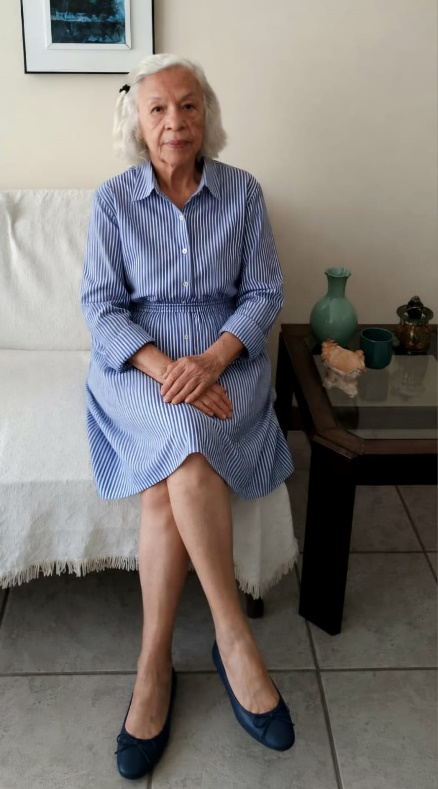
\includegraphics[width=5cm]{media/image1.jpeg}
\caption{Professora Maria Augusta de Araújo Moreno. 
Arquivo pessoal da Prof.\superau  Maria Augusta.}
\end{center}
\end{figure}

Em 1959 foi para Faculdade de Filosofia da Universidade de São Paulo,
onde estudou topologia sob orientação de Omar Catunda e cursou
disciplinas do mestrado com bolsa de pós-graduação. Ao retornar para a
Bahia tornou-se professora assistente do Departamento de Matemática do
Instituto de Matemática e Física (IMF)\footnote{O Instituto de
  Matemática e Física vai ser desmembrado em institutos distintos com a
  Reforma Universitária, em 1968. Em 2023 passa a se chamar Instituto de
  Matemática e Estatística, como o mencionaremos ao longo deste
  trabalho.}, em 1961, onde ofereceu seminários, como o de Topologia
Geral, em 1961.1, e disciplinas no Ensino Superior, como a de Topologia,
em 1964.

No entanto, em função de uma lógica de distribuição do trabalho entre os
professores do IMF, sob a liderança da professora Martha Maria de Souza
Dantas, ela passa a integrar a equipe do Instituto comprometida com o
projeto de modernização da Matemática no Ensino Secundário, ligado ao
Centro de Ensino de Ciências da Bahia (CECIBA) e ao Colégio de
Aplicação, juntamente com as colegas, Eliana Costa Nogueira, Norma
Coelho Araújo, Neide Clotilde de Pinho e Souza, Eunice Guimarães (DIAS,
2002; MENEZES, 2015).

É nesse contexto de atuação, mais especificamente ligada ao Colégio de
Aplicação, que a professora Maria Augusta destaca suas memórias como
docente da UFBA e também é apontada nas memórias dos estudantes como uma
referência de dedicação ao ensino da Matemática, celebrada como uma
agente de modernização dos padrões de ensino da época.

Trazer essas memórias é uma tarefa importante na compreensão do papel do
Instituto de Matemática e Estatística (IME) e de seus professores no
processo de qualificação do Ensino Secundário na Bahia a partir da
década de 1960, merecendo serem revisitadas e comporem a historiografia
da Educação Matemática no estado, tendo o IME como uma instância de
difusão e implementação de padrões modernos que internacionalmente
vinham se estabelecendo naqueles anos.

O Colégio de Aplicação começou a funcionar em 1949 e tinha entre seus
objetivos principais servir de espaço de prática didática para os
estudantes dos cursos de licenciaturas da UFBA, tendo se tornado também
um campo de experimentações educacionais, como costuma ser lembrado por
vários de seus ex-alunos. O Colégio teve suas atividades encerradas em
1976 quando os professores da UFBA que ali atuaram foram realocados em
outras atividades voltadas para o Ensino Superior em diferentes Unidades
da Universidade, como conta a professora Maria Augusta:

\begin{quote}
{[}...{]} \emph{quando o Colégio de Aplicação acabou eu fui chamada pra
ir pro Instituto de Matemática, porque todos professores tomaram seus
destinos, então, pela minha capacidade, pela habilidade, ao invés de ir
para a Educação, porque eu poderia ter ido pra Educação,eu fui para o
Instituto de Matemática} (MORENO, 2012, p. 8)\emph{.}
\end{quote}

Com o retorno às atividades no Ensino Superior, a professora Maria
Augusta seguiu ministrando disciplinas do Departamento de Matemática
para os cursos da Universidade até abril de 1989, quando se aposentou
como professora adjunta (MORENO, 2026).

A seguir, são apresentadas textualizações de trechos de entrevistas
concedidas pela professora Maria Augusta e alguns de seus ex-alunos à
respeito da atuação dela no Colégio de Aplicação, que foram organizados
por tópicos.

\itshape

\section{A chegada no Colégio de Aplicação}

Eu tinha sido aluna do Curso de Matemática na UFBA na época da
professora Martha Dantas, que coordenava o grupo que tinha uma proposta
de criação de materiais ligados à Matemática Moderna. Depois de ter me
formado em Matemática, ou melhor, antes mesmo de me formar, eu já
comecei ensinar no Colégio de Aplicação. Porque eu substituí a
professora Nilza (da Rocha Medrado dos Santos) no terceiro ano de
Colégio porque ela estava grávida e precisava de um professor
substituto. Dos alunos que estavam estagiando eu fui selecionada para
começar a ensinar. Aí fiquei no Colégio de Aplicação até... --- eu não
lembro bem até que ano que eu fiquei --- mas sempre, sempre... é... até
os últimos anos do Colégio.

Como eu disse, eu comecei ensinar no terceiro ano, quer dizer, dei
continuidade às minhas aulas de prática, não é?! Aquela parte ligada ao
Curso de Matemática, depois estive dois anos fora, em São Paulo, na
Faculdade de Filosofia com o professor Edson Faraco que ensinava
Topologia, só depois voltei para a Bahia.

Martha Dantas me acompanhou a vida toda, na Faculdade, na indicação de
cursos, foi ela quem me indicou e tudo, ela me... animou pra ir pro
Colégio de Aplicação. Também me indicava para dar aulas particulares,
então, os resultados que chegavam para ela eram tão bons que ela só
fazia me indicar, só dizia assim: ``pra ensinar só Maria Augusta''. Eu
que já no meu tempo de ginásio dava banca, atuei dando muita aula
particular. A pessoa me procurava e dizia assim: ``olha, Dona Martha
disse que se a senhora não ensinar, ninguém vai dar jeito, se a senhora
não der jeito, ninguém dará mais jeito''.

A minha relação com ela era a melhor possível, porque eu sempre tive
Martha em alto conceito, um conceito muito alto da pessoa dela e da
professora... e, reciprocamente, ela sempre me prestigiou, como eu lhe
disse, me indicando para diversas atividades não só particulares, como
também para a Faculdade, ela me prestigiava muito, muito bom, muito bom
entrosamento.

Martha foi a vários colóquios, sabe?! Portugal, França... Ela viu o que
estava mudando na Matemática, como é que estavam mudando e... ela se
pautou nisso e, juntamente com o professor Catunda, começaram a elaborar
o material relativo à Matamemática Moderna.

Sobre minha atuação como professora... eu era muito rigorosa, eu tinha
uma... uma característica que eu apliquei no Colégio de Aplicação e no
João Florêncio Gomes\footnote{Outra escola de Salvador em que a
  professora Maria Augusta atuou.}, eu fazia teste todo santo dia, hoje
eu dava a matéria, hoje eu dava o assunto, amanhã eu já aplicava o
teste. Todo santo dia. São... eram perguntas bem simples, imediatas, se
eu hoje falava sobre translação, explicava translação, dava exemplo,
amanhã eu já anotava no teste, ditava, dividia a turma em quatro, sem
que eles pudessem ver o que o outro estava fazendo, sem eles poderem
pescar, né?! E... eles ficavam a princípio meio tensos porque achavam
que não ia dar tempo, mas foi um sucesso porque quando chegava na hora
da prova era só rever e porque todo santo dia eles tinham obrigação de
ler a matéria.

\begin{figure*}
\begin{center}

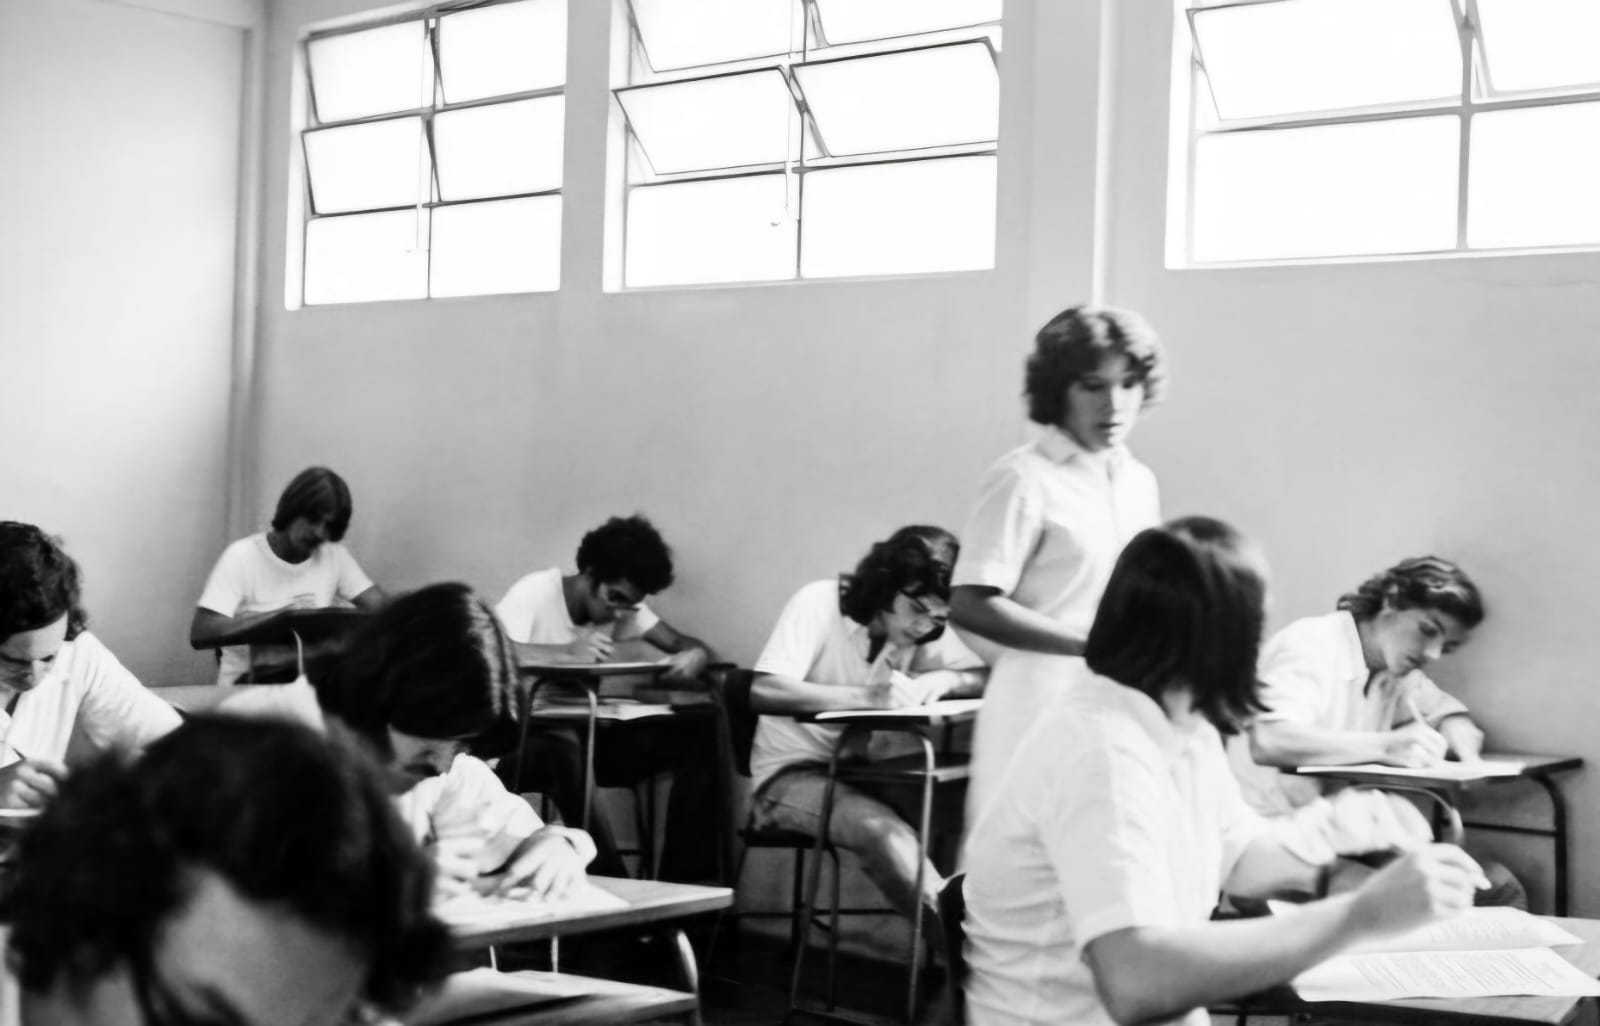
\includegraphics[width=5.14783in,height=3.30032in]{media/image2.jpeg}
\end{center}
\caption{Prof.\superau  Maria Augusta na sala de aula do CA. 
Arquivo pessoal da Prof.\superau  Maria Augusta.}
\end{figure*}

\section{Sobre a Matemática Moderna no \\Colégio de Aplicação}

A experiência de estar lançando uma coisa nova no seio da Matemática, no
meio do Colégio, isso pra mim era empolgante, né?!

Na parte de álgebra, veja só, juntamente com o livro que foi dado pelo
professor Catunda, com a orientação do professor Catunda, por falta de
materiais prontos, comecei usando no Colégio de Aplicação um livro que
era uma tradução de um livro Americano\footnote{A professora se refere
  ao livro de Matemática que foi produzido no âmbito de projetos que
  propunham reformar o ensino médio norte-americano, School Mathematics
  Study Group (SMSG). Além da Matemática, também circularam no Brasil
  livros desses projetos ligados a outras disciplinas, como Física,
  Biologia e Química (OLIVEIRA FILHO, 2009).}.

Isso aconteceu antes da experiência de professor Catunda e Martha
Dantas, foi aí que eu introduzi esse livro, foi um achado pra mim, ele
era coisa bem moderna, bem moderna mesmo e não tinha essa conotação de
livro de 1\superou  ano de ginásio, 1\superou  ano de colégio 1\superou , 2\superou  e 3\superou  anos, não. Ele
tinha todos os assuntos, e eu abordava os assuntos de acordo com a nossa
programação.

Sei que era vermelho, o livro e era grosso, a encadernação era muito
boa. O grupo de alunos que eu introduzi esse livro, esse grupo foi um
dos primeiros, pena que eu não tenha ninguém assim pra quem eu possa
apelar à memória. Ele foi usado nos primeiros anos que eu ensinei no
Colégio de Aplicação, não é dizer que no Colégio de Aplicação não
existia, estou lembrando de quando eu estreei no Colégio de Aplicação
com esses materiais, já depois que voltei para a Bahia.

Não era aquilo tradicional, era uma coisa que eu --- não nego, não, --- eu
tinha que estudar, amadurecer... mas, eu amadurecia com eles, porque não
havia tempo pra amadurecer. O Catunda, que era o pai da ideia, ele...
como é que se diz, orientava essa proposta.

Esse livro quando nós estudávamos, por exemplo, a função, ele fazia pela
translação, pela homotetia, mas ``não dava os nomes aos bois'', então,
eu carreguei comigo essas noções. Era um livro cujo autor eu não me
lembro agora, mas ele estudava, primeiramente, por exemplo, a função
identidade, depois ele fazia homotetia, era a questão linear, depois ele
fazia translação, então, você tinha a função de 1\superou  grau. A função de 2\superou 
grau, ele começava pela função, a função era a fundamental, era
``x\textsuperscript{2}'', depois ele fazia homotetia, quer dizer, ele
fazia uma parábola... depois fazia homotetia de acordo com o coeficiente
de A, ela abria ou ela reduzia, levando em conta o sinal. Depois uma
translação, quer dizer, ela deixa de ter o vértice na origem e passa a
ter para cima ou para baixo. Uma translação. Depois... dada uma função
qualquer, como você trabalhar na função do 2\superou  grau para descobrir que
homotetia e que translações foram feitas da fundamental pra se chegar
aqui...

Esse livro abriu muito a minha cabeça e abriu também a dos alunos.
Depois é que eu fui casar que era uma homotetia, era uma translação, e a
simetria também. Até simetria também. Tal função é obtida dessa forma...
fazendo isso, fazendo homotetia, fazendo translação, depois simetria em
relação ao eixo ou em relação ao eixo das ordenadas ou em relação a uma
determinada reta... e aí pronto.

Simultaneamente a esse trabalho, existia lá em Porto Alegre uma
professora que tava fazendo umas experiências, uma maneira de introduzir
os assuntos, mas ela não teve o sucesso esperado por falta de estímulo
para os professores...

Mas, esse livro, uma espécie de uma tradução de um livro americano,
era... era uma coisa! Eu ficava encantada, a maneira não só como
expunha, como ele introduzia a matéria, mas também a maneira como ele
cobrava. Eu me lembro perfeitamente da maneira como ele cobrava, ele
parecia... --- porque americano tem essa... --- parecia que era muito
fácil no começo, depois que você ia ver o perigo que era a maneira como
ele cobrava.

A experiência do uso desse material americano foi interrompida no
Colégio porque veio o projeto de Martha, aí me convidaram para aplicar e
eu aceitei. Era uma proposta diferente: começa que ela introduzia essas
transformações basicamente na geometria; depois é que nós começamos a
introduzir essas transformações na aula, na função e tudo mais,
entendeu? Nesse livro que eu lhe falei antes não citava explicitamente
as Transformações, não.

Depois de um tempo, como eu me dava muito com uma das autoras da equipe
desse outro livro\footnote{CATUNDA; DANTAS, \emph{et al}., v. I, II,
  III, IV, 1971.}, cuja autoria é de Omar Catunda, começaram a querer
experimentar esses materiais, esse livro, e me confiaram. Então, eu
acompanhei uma turma com essa apostila que era, vamos dizer assim, feita
grosso modo. Nós trabalhávamos, eu e ela trabalhávamos, vamos dizer
assim, à tarde e à noite e, de manhã, já estávamos aplicando. Foi muito
assim ``em cima da perna'', então, levei aqueles meninos até o terceiro
ano. Lá eu tinha muita autonomia para agir, não tinha problema, não.

Eu estava comentando com a Neide (Clotilde Pinho e Souza), que na época
em que esses materiais estavam sendo feitos eu já estava simultaneamente
aplicando no Colégio de Aplicação.

Apesar deles não terem o material suficiente, porque se tratava de uma
experiência, então você não encontrava aquela matéria em lugar nenhum,
era só mesmo aqueles apontamentos feitos, folhas assim... que eu
entregava pra eles e aquele material é que eles estudavam, que eles
aplicavam. Depois é que foi feito uma apostila ``grosseira'' e depois é
que eles fizeram um livro de editora, editora tal da Universidade. Mas
foi feito inicialmente assim.

Antes dos livros tinha muito material mimeografado. Era assim: hoje eu
sabia que eu ia dar certo assunto, aí na noite anterior eu preparava o
\emph{stencil} e no dia seguinte, enquanto eu estava dando aula, o
material ``estava batendo'' \footnote{Uma expressão que era muito usada
  para se referir a fazer cópias de um documento no mimeógrafo,
  registrado originalmente no papel \emph{stencil}.}. Em seguida, o
rapaz levava para mim na sala e eu entregava para poder ter maior
fixação, né?! Eu cobrava muito, mas muito mesmo deles. Eles ficavam
``meio esticados'' com tanta coisa, até porque o Colégio não era fácil,
viu?! O Colégio puxava muito. A professora de história não deixava
escapar, era Matemática de um lado, História de outro, Português do
outro... cada um puxava para o seu lado.

Quando chegaram o livros onde foram dadas as Transformações, então
encaixou, aquilo era apresentado num crescendo... Pode até ser que
alguém dissesse: ``Ah! mas eu achava que a outra maneira era mais
simples, era mais imediata''; eu digo uma coisa: ``mas aí você não
teria, de maneira nenhuma, a visão de como aquilo se passava''. E isso
depois se estendia para ensinar todas as funções, trigonométricas,
logarítmicas, exponenciais...

Omar Catunda era o nosso coordenador, ele foi nosso diretor no Instituto
de Matemática --- não sei lhe precisar quanto tempo ficou na direção.
Depois se aposentou, se afastou, mas continuou a orientar esse trabalho
que Martha redigiu. Ele não ia mais, mas ele dava orientações. Nós nos
reuníamos na residência de Martha e não tínhamos horário de saída, só de
chegada. A gente ia se entusiasmando, a gente ia ficando, ficando... era
lá na casa dela na Graça porque, na verdade, nós éramos funcionárias do
governo e tínhamos esse privilégio de fazer esse trabalho, e como era
difícil encontrar uma sala onde nós nos reuníssemos e tivéssemos
tranquilidade total, ela puxou para casa dela.

Ela era a mais velha e puxou para casa dela. Mas, era mais rigorosa do
que qualquer chefe de departamento, qualquer chefe de faculdade, ela era
muito séria e nós retribuíamos, né?! Todo dia em vez de ir para outro
lugar, íamos pra casa dela. O trabalho era feito lá.

Então, eu mesma não tenho assim aquela vaidade, aquela pretensão de ter
feito... de aplicar método A, método B, meu negócio era... o meu intuito
era estudar com eles, era fazê-los entender como eu estava entendendo
aquilo, porque não tinha tempo nem de amadurecer. Eu... eu gostava da
experiência em si, eu gostava! Mas, dizer que eu tinha conhecimento
completo, eu não tinha nem... pra falar francamente, eu não tinha nem
consciência de que a matéria seria dada para eles na universidade, mas,
depois é que eu fui saber que era... que constituía a matéria de
Geometria Analítica e, também da parte moderna, que eles já começavam
comigo, não era na faculdade, não.

Eu não tinha total consciência do bem que a aplicação daquelas apostilas
ia fazer porque... Quando eles entraram na faculdade já deslancharam,
porque o vestibular para eles foi considerado facílimo e as matérias
tinham a ver com a matéria que eu ensinei, que estava associada à
Matemática Moderna.

\begin{figure*}
\begin{center}

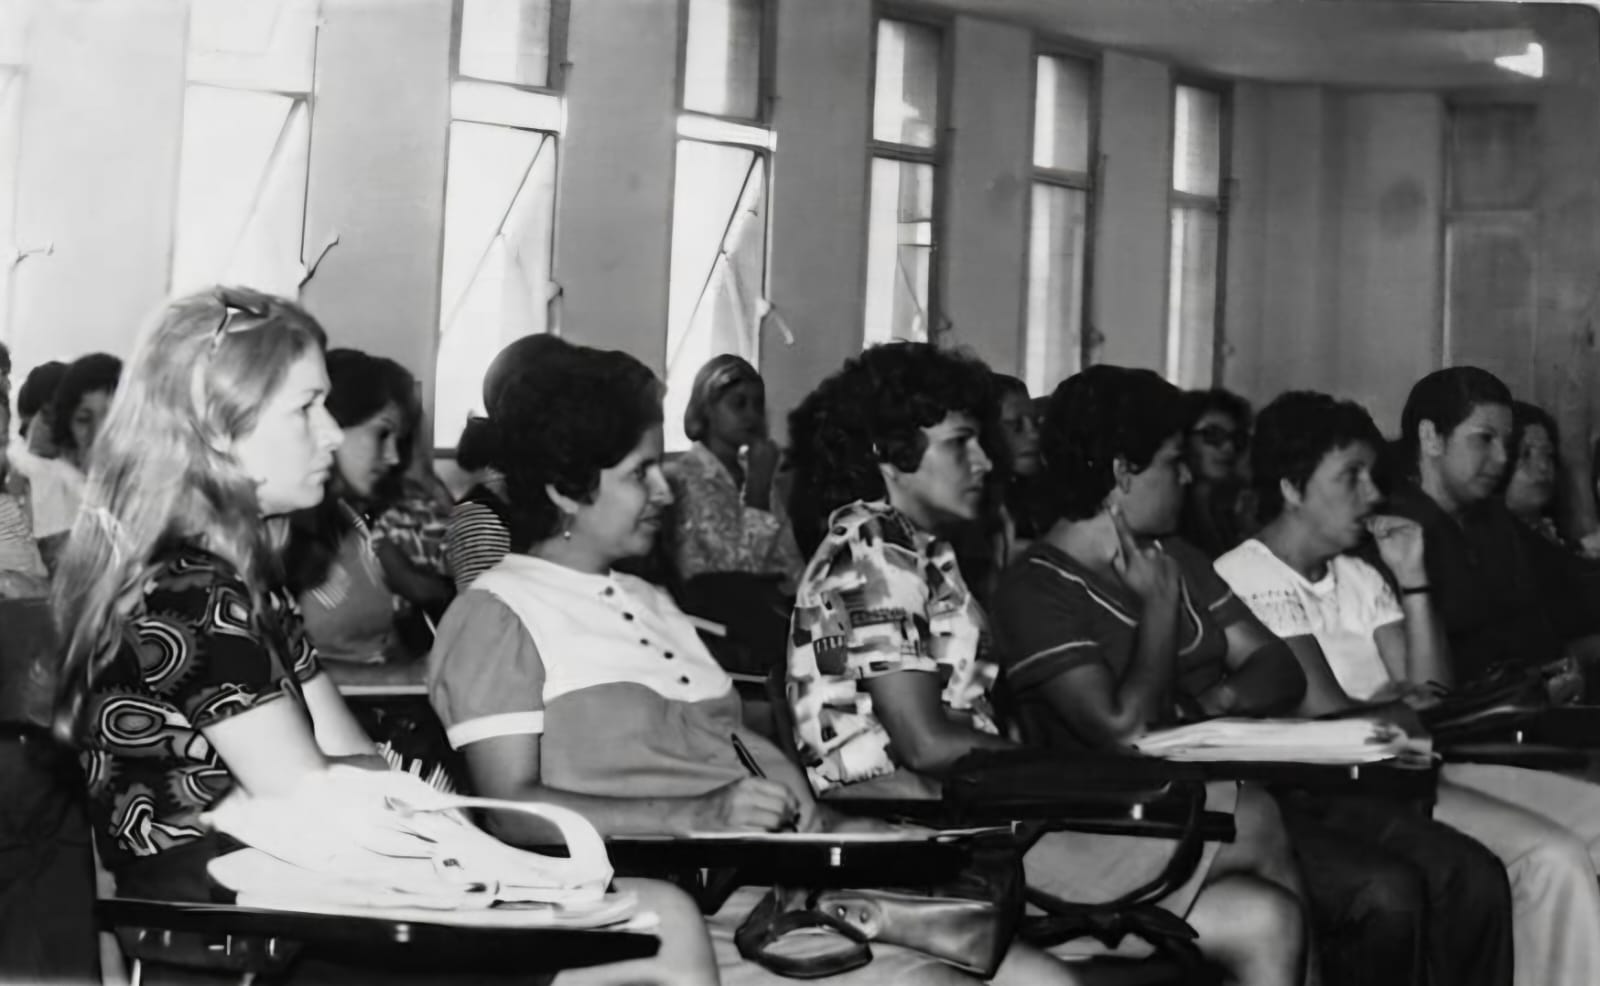
\includegraphics[width=5.1237in,height=3.15652in]{media/image3.jpeg}
\end{center}
\caption{Registro do 3\superou  Seminário de Pedagogia da Matemática, que
ocorreu em Salvador, de 8 a 15 de agosto de 1973. A prof.\superau  Maria Augusta
está na primeira fila, no centro da foto com camisa estampada. Arquivo pessoal da Prof.\superau  Maria Augusta}
\end{figure*}


Foi o professor Catunda que introduziu no Colégio de Aplicação a noção
de Estatística, a noção de Financeira e a noção de Derivada, que não se
usava, né?! Não se dava, não. No livro do 3\superou  ano tinha Derivada,
Financeira e Estatística. Não precisava ser com profundidade, mas uma
espécie de apresentação e você vê que tanto valeu que entrou no programa
do vestibular, não foi? Ele tinha uma visão muito além, apesar de ser
uma pessoa de idade, ele tinha uma visão muito grande. Não precisava
ficar se aprofundando em coisas que eles poderiam ver depois, não era
essa a pretensão dele. A pretensão era que tivessem uma visão geral
desses assuntos. Quem é que estudava Financeira antes? Nunca, nunca ouvi
dizer, mas foi lá que foi introduzida Financeira, Estatística e
Derivada. Derivada? Derivada no 3\superou  ano! É uma coisa também que eles
foram ver logo no começo do estudo de Cálculo, né?!

Eu falei da Geometria Analítica, que eles viram... translação, simetria
e homotetia, mas a parte de Álgebra, a parte de Cálculo nós
introduzíamos no 3\superou  ano do Colégio.

Se você me perguntasse qual a principal mudança trazida pela Matemática
Moderna eu diria que era a inserção do conteúdo, mesmo. Porque até
então, mesmo quando eu estudei, não se falava em conjuntos, aquela
teoria do conjunto todo... e lá no Colégio de Aplicação nós começamos a
estudar todo conteúdo pela teoria dos conjuntos.

E isso mudou, inclusive, a maneira deles estudarem, não só no ginásio
como no colégio, no colégio principalmente. Facilitou muito mais o
aprendizado. Foi muito eficiente pra eles, em vez de ser aquele conteúdo
tradicional. Nós estudávamos tudo, mas a maneira de introduzir, a
maneira de cobrar também era diferente. Então, na minha maneira de ver,
acho que facilitou pra eles terem estudado a parte da teoria dos
conjuntos, né?! e como também as modificações na parte de Geometria,
Geometria principalmente, facilitou muito.

O estudo da Geometria no Colégio era todo feito através da Geometria das
Transformações. Eu sempre estudei formalmente os polígonos,
quadriláteros... tudo, tudo através da simetria ou então da homotetia,
até Geometria no espaço. Foi muito... abriu muito, sabe?! E abriu
facilitando, não abriu complicando esses estudos, não, abriu
facilitando. Com a maturidade e os conhecimentos anteriores que eu tinha
isso só fez ajudar e pra quem não conhecia de outra forma era muito mais
fácil aprender, muito mais fácil. De modo que pra mim foi muito
gratificante.

Demonstrações a gente fazia tudo baseado nas Transformações. Mas, aí
entrava um fator: a minha dificuldade de me adaptar, porque... eu
estudei o processo tradicional, né?! E pelas Transformações era muito
simples, às vezes, eles que puxavam... tiravam a conclusão mais rápido
do que eu, porque eu tava ``caducando já naquele assunto'', né?! Tava
usando sempre coisas mais complicadas e pelas Transformações
simplificava tudo.

O que foi um pouquinho chato para mim é que eu ensinava no Colégio
Aplicação e no João Florêncio Gomes. Dava vontade de levar essa proposta
para lá também, mas não podia por causa do material. O material estava
todo ``preso'' à proposta do Colégio de Aplicação. Não podia fazer.
Então, eu fazia lá de uma forma e no João Florêncio de outra.

Eu não entendo a dificuldade que existiu de aplicar aqueles livros nos
diversos colégios onde depois foram feitas iniciativas semelhantes. Acho
que não tinha a ver com o Colégio de Aplicação. Mas, Dona Martha como
parte do estudo sobre aquela proposta levou para outros colégios e foi
bem difícil, não sei se falta de base, preparo ou mesmo coragem do
professor para aplicar.

O que mais eu lamento é o Colégio ter acabado. Parece que a Universidade
achava um desperdício que professores que recebiam um salário de
professores da universidade estivessem trabalhando em um colégio de
ginásio e, por conta disso, o reitor achou por bem fechar. Foi na época
da professora Zilma (Parente de Barros). Foi ela que deu por terminado,
né?! Foi na gestão dela que o Colégio acabou. Eu acho que a decisão foi
de ordem financeira. Agora, se olhassem para o outro aspecto, para a
sociedade, não tinha coisa melhor.

\section{O retorno ao %trabalho
Ensino Superior}

Já na Faculdade quando eu voltei... eu ensinei uma matéria que não
existe mais, que era uma espécie de recuperação. Era assim: você entrava
no curso de Matemática com uma nota de entrada no curso, com uma nota de
Matemática fraca, aí a Universidade dava um ``curso de recuperação'', em
que me foi pedido para explorar Geometria, Trigonometria e... essas
matérias assim, para ver se melhorava o nível, mas, não deu muito certo,
não, porque não continuou.

Hoje em dia acho que entra pesado nas matérias de Cálculo, Geometria
analítica... entra pesado, não tem mais isso, não, mas levou-se alguns
anos, eu não sei se foram dois ou três anos com essa experiência. Esse
curso, apesar de ter esse conceito: ``ah, é recuperar os alunos que
tiraram nota baixa, que não atingiram o certo nível em Matemática...''
tive alunos que eram ótimos.

O curso se chamada Complementos de Matemática e era uma espécie de
revisão do Curso de Científico para que os alunos enfrentassem melhor a
faculdade. Mas, também tinha aquele aluno que já se achava capacitado
para enfrentar a Matemática e tudo mais. Mesmo assim tinha que tolerar
uma pessoa fazendo revisão, coisa que ele já tinha feito no cursinho,
coisas muito melhores, talvez. Aí eu tive que fazer alguma coisa
diferente, né?! Dialogar e discutir umas questões, botar uns problemas
difíceis para resolver e tudo... mas, terminou.

Depois foi que eu comecei a ensinar disciplinas de Cálculo. Ensinei
Cálculo 1, Cálculo 2, só não cheguei a Cálculo 3, nunca peguei uma turma
de Cálculo 3, só Cálculo 1 e Cálculo 2.

\section{Lembrando da Professora: memórias de ex-alunos de Maria Augusta}

\upshape
Segue a textualização de uns poucos trechos de entrevistas de ex-alunos
da professora Maria Augusta no Colégio de Aplicação. Esses trechos são
bem emblemáticos da atuação dela, reforçando as memórias dela sobre o
trabalho que realizou ou indicando o modo como ela ficou marcada na
memória deles.
\itshape

\begin{figure*}
\begin{center}

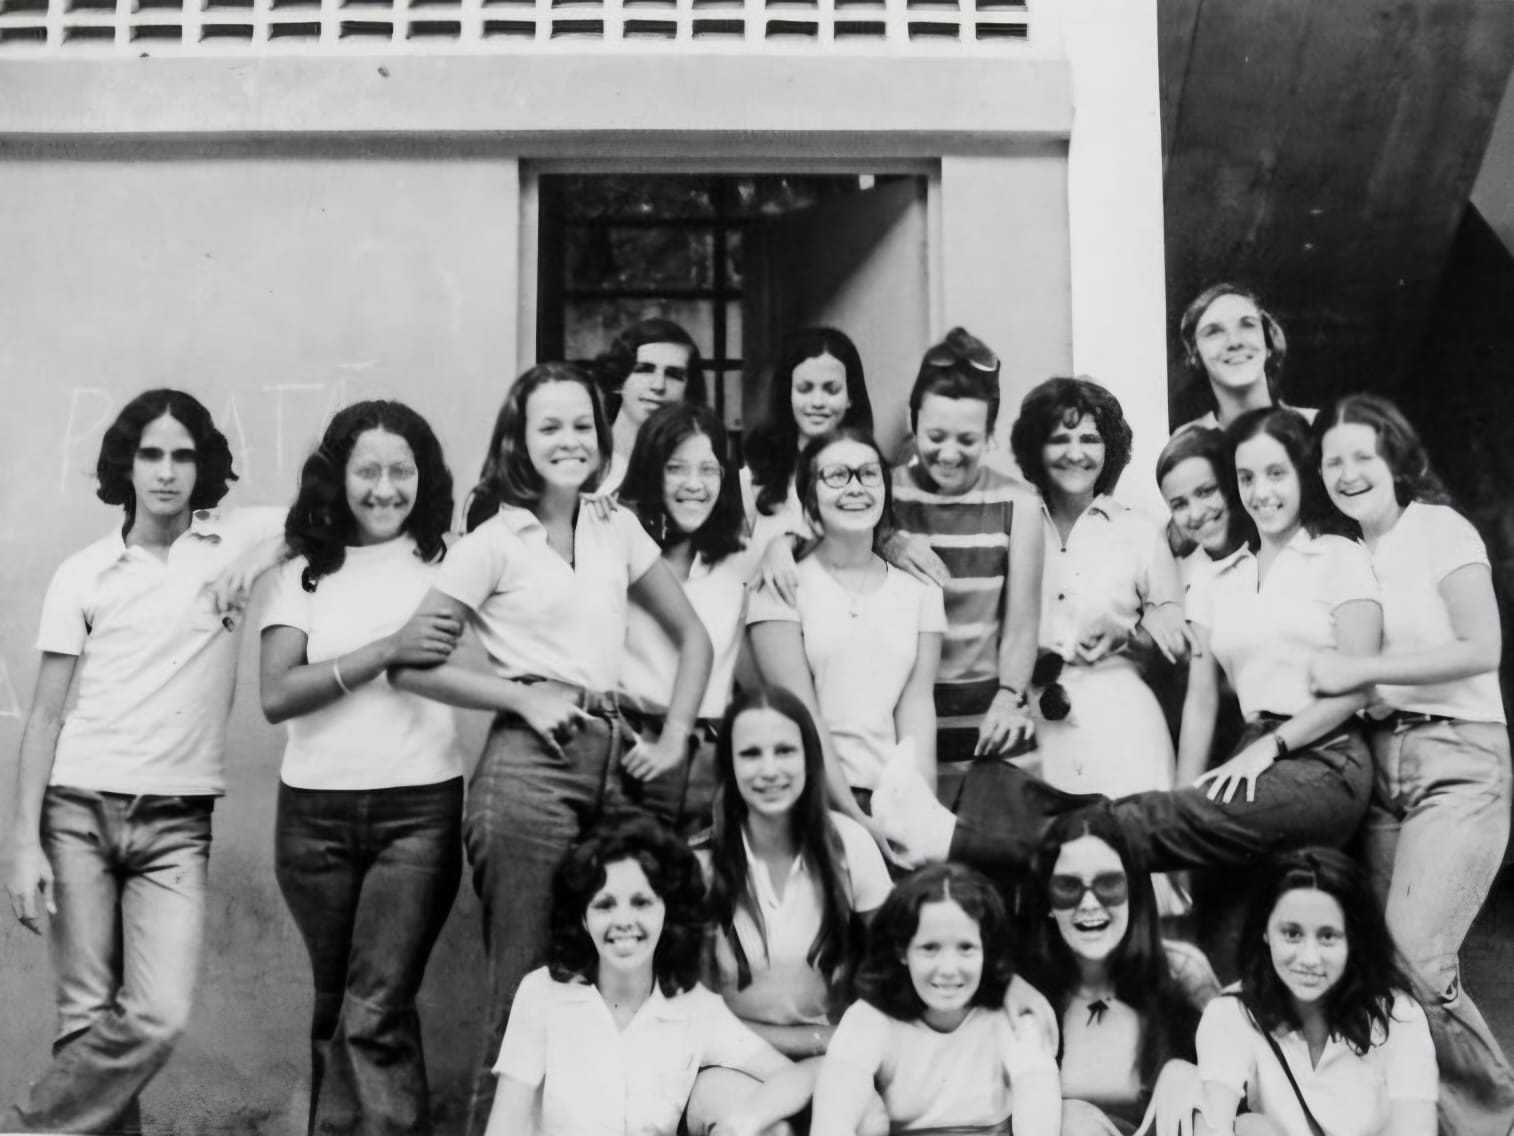
\includegraphics[width=12cm]{media/image4.jpeg}
\end{center}
\caption{A prof.\superau  Maria Augusta entre os estudantes do CA. Arquivo pessoal da Prof.\superau  Maria Augusta.}
\end{figure*}

\paragraph{Jaci Maria Ferraz de Menezes}\footnote{Ingressou no CA em 1961.}
Quando Maria Augusta começou a trabalhar com a nossa turma, eu acho que
já na primeira unidade ela trabalhou com algumas apostilas com teoria de
conjuntos. É uma lembrança fugaz --- eu acho que era só para ela dar uma
``agilizada nos conceitos'', no início.

Dona Martha (Dantas) era assim, aquela senhora imponente, sempre de
salto alto, certo?! E que estava presente todo o tempo na vida do
Colégio e... Maria Augusta era baixinha, um pouco menor, e, assim, ela é
elétrica, ``The Flash''. Ela entrava na sala de aula, ela não fazia mais
chamada, então, ela deixou pra lá. ``Bom dia, bom dia, bom dia...'',
passava para o quadro de giz e passava uma lista de exercício e começava
o trabalho, a fazer exposição e, depois, começava o trabalho todo, com
exercícios, etc.

``Guguta'' se lembra de uma resistência à implantação das atividades de
Matemática por parte de uma colega que fumava --- nós, na época, as
meninas na sala, ninguém fumava na sala, era proibido, mas no intervalo
podia fumar, nos corredores não tinha maiores restrições ---, então, o
pessoal tava na porta da sala esperando ela chegar aí, na hora que ela
chegou, essa colega encheu o pulmão e soltou a fumaça no rosto dela. Ela
ficou ofendidíssima, se sentiu agredida, ela se lembra até hoje! Ela
perguntou pra mim dessa vez que a gente se encontrou, em dezembro do ano
passado: ``como era o nome daquela sua colega...'' eu disse: ``eu não me
lembro, Maria Augusta''. ``Ah, pois ela encheu o pulmão e soltou a
fumaça na minha cara.''

Pense numa barreira, assim, uns três ou quatro, na hora dela entrar na
sala... porque, justamente, esse pessoal tava que não aguentava mais a
Matemática no regime linha dura de Maria Augusta. No ano seguinte eles
passaram para o Clássico. Mas, ela fazia com muita naturalidade... não é
livrando a cara dela, não, ela fazia com muita simpatia, ela dava aula,
fazia, preparava... e o pessoal aprendia, tanto assim que eu que não sou
do ramo ainda me lembro.

\paragraph{Anônima}\footnote{Ingressou no CA na turma de 1963.}
Como é que a gente aprendia a demonstrar na escola? Não sei como a gente
aprendia a demonstrar na escola, não sei, mas se você conseguir um livro
da época, você pode ver que tudo tem demonstração, tudo tem hipótese,
tese, demonstração. Se fazia, se fazia.

Outro dia eu perguntei a Maria Augusta: ``Maria Augusta, como é que você
enfiava aquilo tudo na cabeça da gente?'' e ela respondeu: ``também não
sei, eu também não sei''. E a gente aprendia, a gente aprendia.

Não era Geometria tradicional, não, era com rotação, simetria,
translação e a geometria plana era toda com base nas transformações
lineares, nas transformações no plano. Maria Augusta era professora de
Matemática que aplicava.

Tudo, tudo, tudo mesmo, que você possa imaginar em trigonometria, era
dado. A gente saiu do Aplicação com Limite, Derivada e Integral,
perfeita. Teoremas e tudo! Saí de lá completa. Eu saí do Colégio direto
para a Universidade. Terminei em meia nove e, em setenta, eu tava
cursando (Matemática).

\paragraph{Raimundo Mesquita de Luna Freire}\footnote{Ingressou no CA na
  turma de 1966. A entrevistada preferiu não ser identificada,
  preferindo a utilização deste pseudônimo.}
Durante os meus sete anos no Colégio, somente em um deles, o segundo
ano, é que eu tive uma outra professora, durante seis dos sete anos a
professora foi Maria Augusta Moreno. Ela era uma das professoras que,
junto com o professor Omar Catunda, desenvolvia aquela metodologia que a
gente estudava.

O que eu me lembro é que ela era uma pessoa altamente comprometida,
muito bem preparada, que sabia a matéria que ensinava e sabia
transmitir. Eu imagino que ensinar aos meninos de doze, treze anos, você
sendo uma professora que, inclusive, dá aula na universidade, isso aí
exige uma habilidade específica e ela tinha. Então, ela tinha tanto
conhecimento naquilo que ia ensinar quanto uma facilidade de transmitir.

Ela tinha uma didática muito boa. Era uma pessoa muito rígida e
inflexível, que não dava essa abertura para contestar, nem pra tirar
dúvidas, pelo menos essa era minha sensação, e era uma sensação
generalizada, pelo que eu sei, não era só minha, não, era uma sensação
generalizada, mesmo para tirar dúvida. Você tinha medo de dizer ``não
entendi, pode explicar...'' claro que existia essa possibilidade, não
era um regime ditatorial, mas tinha uma barreira grande que eu não tinha
com outros professores, para você ver que não era uma regra da Escola,
era uma coisa muito da personalidade dela, tinha professores até
piores...

Outra coisa que eu tô me lembrando agora... a avaliação normalmente era
um teste e uma prova à cada unidade, além disso, tinha um ``testezinho''
praticamente todo dia de aula, tinha um teste de uma única pergunta no
início da aula. A gente tinha uma cadernetazinha, todo mundo tinha que
ter uma caderneta dessa, então, no início da aula ela passava uma
pergunta, só um problema rápido, que você tinha que resolver em dez ou
quinze minutos e, aí, no fim da unidade, a soma desses vários pequenos
testes valia uma nota também, igual à nota do teste e da prova. Acredito
que era uma forma de obrigar a tá em dia com a matéria, né?!

Essa cadernetinha ficava com a gente. Era assim, você levava sua
caderneta, ela passava o problema, você resolvia ali e entregava para
ela na mesma hora. No mesmo dia ela devolvia, já com a sua nota, né,
como era só uma questão, era ``um certo'', ``um errado'' ou ``um meio
certo'', sei lá... mas ela devolvia no mesmo dia que você levava, então,
só ficava com ela para corrigir. Foi o que eu disse, acho que a ideia
era obrigar a ficar em dia com a matéria, para que você não acumulasse
para a véspera da prova, né?! Você tinha que estar em dia com a matéria.
Em geral, essas questões não eram questões muito difíceis, até porque
você tinha pouco tempo para resolver, era mais objetiva mesmo, sobre o
que tinha sido dado na última aula.

\paragraph{Valber Roberto Carneiro Carvalho}\footnote{Ingressou no CA em
  1971 e teve que sair após a 8\superau  série por não serem mais oferecidas
  novas turmas para o Segundo Grau (atendendo ao processo de redução de
  turmas em função do fechamento do CA, que se deu em 1976).}
Quando chegamos na sétima série, sétima e oitava, nós tivemos o prazer
de estudar, de sermos alunos de uma mulher... uma das autoras do livro
que a gente estava estudando, você imagina o que significa isso? Maria
Augusta. O livro era feito por oito pessoas, o primeiro, o mais famoso,
um ``matemático daqueles'' chamado Omar Catunda, e ela era a última ou a
penúltima. Rapaz, aquilo era um delírio pra gente, a mulher era uma das
autoras do livro que a gente tava estudando!

Você conversava com gente, com seus colegas de outros colégios... o
livro de Matemática que a gente estudava tinha nossa professora como uma
das autoras!

As provas dessa professora, Maria Augusta, eram assim: ``Considerando
que existem duas retas paralelas que cortam outras duas retas --- não sei
o que lá... --- e que o ângulo tal S1 é igual... congruente com o ângulo
tal... prove que essa terceira reta que passa aqui é paralela também a
essa duas''. Você tinha que provar por lógica geométrica. ``Com
efeito...'' --- a gente tinha que começar assim ---, ``com efeito,
considerando-se que o ângulo tal é igual ao ângulo tal e que o teorema
de não sei quem diz que quando duas retas se cruzam no ângulo tal
pa-pa-pa... gera uma terceira reta não sei o quê...''

Então, para você responder aquilo você escrevia um catatau de treze
linhas, justificando... até você provar por A mais B, por lógica, que
aquele ângulo tal era igual ao ângulo tal. A prova de matemática da
oitava série, era assim, era uma prova muito difícil, tinha que
escrever, que relacionar teoremas e gerar conclusões, lhe colocava para
pensar.

Isso era a Matemática da 8\superau  série! Isso mexia com a gente pra caramba e,
confesso a você, tinha uma certa dificuldade, não era um terreno em que
eu bailava... eu tinha que fazer uma explanação sobre a Matemática,
porque que isso é igual a isso e porque isso é simétrico a isso. Eu
tinha que usar a lógica, os teoremas, usar as teorias da Matemática pra
chegar ao resultado desejado, entendeu?! Isso não era mole, não, você
escrevia muito, você saía de cuca fundida das provas.

Ela inventou um sistema de avaliação em que o aluno tinha que estar
presente no início da aula, você não podia faltar e não podia perder o
início da aula porque havia um teste, ela chamava de miniteste ou
``testinho''. Para ninguém ``pescar'' ela dividia a sala em quatro
diferentes turmas com testes diferentes e, então, ela dava quatro
exercícios, um para cada uma dessas turminhas responder, aí você
respondia e ela recolhia em cinco minutos.

Quando você acertava recebia um ``mais'' e se errasse recebia um
``menos''. A quantidade de ``mais'' que você tivesse era somada e aquilo
gerava uma nota que ia ser combinada com a nota da prova, e aquilo era
um terror de alguma forma, mas também te mantinha aceso, é como um
piloto de avião que tem que fazer teste todo mês para saber se está bem.
Só que era toda aula, e foi um período, muito, mas muito difícil, eu fui
muito bem na sétima série, eu me lembro, em equações do segundo grau e
sofri um pouquinho na oitava, que era Geometria.

\upshape

\sepdecorada

Quando realizei entrevistas com ex-alunos do Colégio de Aplicação a
professora Maria Augusta foi a professora que mais figurou como
associada ao projeto de modernização da Matemática liderado por Martha
Dantas e Omar Catunda.

As marcas que ela deixou na memória de seus alunos lhe deram um certo
destaque, seja pelo grau de comprometimento com o ensino de Matemática,
seja pelas mudanças que aquele projeto representou na formação acadêmica
deles, repercutindo na trajetória profissional mesmo daqueles que não
seguiram carreiras ligadas às exatas.

Enfim, este artigo trouxe memórias ligadas à trajetória profissional da
própria professora Maria Augusta de Araújo Moreno e uma seção com
recortes de memórias de alguns ex-alunos dela no Colégio de Aplicação.

Podemos concluir afirmando que com este trabalho se destacou um perfil
de professores do IME que, desde o começo do Curso de Matemática,
enfocaram sua atuação na qualificação ensino de Matemática na Educação
Básica baiana, que acompanharam o trabalho iniciado pela professora
Martha Maria de Souza Dantas, nossa personagem mais renomada nesse campo
de atuação do Instituto.

\section{Bibliografia}

CATUNDA, O.; DANTAS, M. M. S. \emph{et al.} \emph{Ensino atualizado da
matemática 1}: curso ginasial. Vol. I, São Paulo: EDART, 1971.

\_\_\_\_\_\_. \emph{Ensino atualizado da matemática 2}: curso
ginasial. Vol. II, São Paulo: EDART, 1971.

\_\_\_\_\_\_. \emph{Ensino atualizado da matemática 3}: curso
ginasial. Vol. III, São Paulo: EDART, 1971.

\_\_\_\_\_\_. \emph{Ensino atualizado da matemática 4}: curso
ginasial. Vol. IV, São Paulo: EDART, 1971.

OLIVEIRA FILHO, F. \emph{O School Mathematics Study Group e o
Movimento da Matemática Moderna no Brasil}. 2009. 201.f Dissertação
(Mestrado em Educação Matemática) -- Universidade Bandeirante de São
Paulo, São Paulo.

DIAS, A. L. M. \emph{Engenheiros, Mulheres, Matemáticos}: interesses e
disputas na profissionalização da matemática na Bahia (1896 -- 1968).
São Paulo, 2002. 320 f. Tese (Doutorado em História Social) --
Universidade de São Paulo.

MENEZES, M. B. \emph{A Matemática das Mulheres}: as marcas de gênero
na trajetória profissional das professoras fundadoras do Instituto de
Matemática e Física da Universidade da Bahia. (1941-1980). Salvador,
2015. 381f. Tese (Doutorado em Estudos Interdisciplinares sobre
Mulheres, Gênero e Feminismo) -- Universidade Federal da Bahia.

MORENO, Maria Augusta de Araújo. \emph{Entrevista}. Salvador, 13 fev.
2012.

MORENO, M. A. A. \emph{Ficha Funcional}. Salvador, Arquivo da
Pró-Reitoria de Desenvolvimento de Pessoas da Universidade Federal da
Bahia (PRODEP-UFBA). Acesso em 18 jun. 2026.

RIOS, D. F. \emph{Memórias de ex-alunos do Colégio de Aplicação da
Universidade da Bahia sobre o ensino de Matemática Moderna}: a
construção de uma instituição modernizadora. 2012. 505 f. Tese
(Doutorado em Ensino, Filosofia e História das Ciências) -- Universidade
Federal da Bahia, Universidade Estadual de Feira de Santana, Salvador,
2012.

\end{document}
